\documentclass[a4paper,titlepage]{scrartcl}
\pagestyle{plain}
\usepackage[utf8]{inputenc}
\usepackage[T1]{fontenc}
\usepackage[german]{babel}
\usepackage{units}
\usepackage{floatrow}
\usepackage{amsmath,amssymb,amstext}
\usepackage{pgfplots,pgfplotstable}
\usepackage{numprint}
\usepackage{graphicx}

\newfloatcommand{capbtabbox}{table}[][\FBwidth]
\numberwithin{equation}{section}

\title{Auswertung vom Versuch P2-23: Laser B}
\author{Gruppe Di-22\\Jonas Müller, Genti Saliu}
\date{15. Mai 2014}

\begin{document}

\begin{titlepage}
\maketitle
\thispagestyle{empty}
\end{titlepage}

\newpage
\pagenumbering{roman}
\tableofcontents

\newpage
\pagenumbering{arabic}

\section{Spaltversuch}
Dieser Demonstrationsversuch wurde mit den anderen Gruppen gemeinsam und mit Unterstützung der Betreuerin durchgeführt. Es wurde die Beugungsfigur eines Einzalspats mithilfe eines Phototransistors gemessen. Der Phototransistor wurde rechnergesteuert mit einem Schrittmotor durch die Beugungsfigur geführt und hat Intensitäten an verschiedenen Stellen gemessen. Ein Analog-Digital-Wandler sorgte dafür, dass die Messdaten auf dem Rechner übertragen und dort gespeichert wurden.
\begin{figure}[H]
	\centering
	\begin{tabular}{@{}r@{}}
		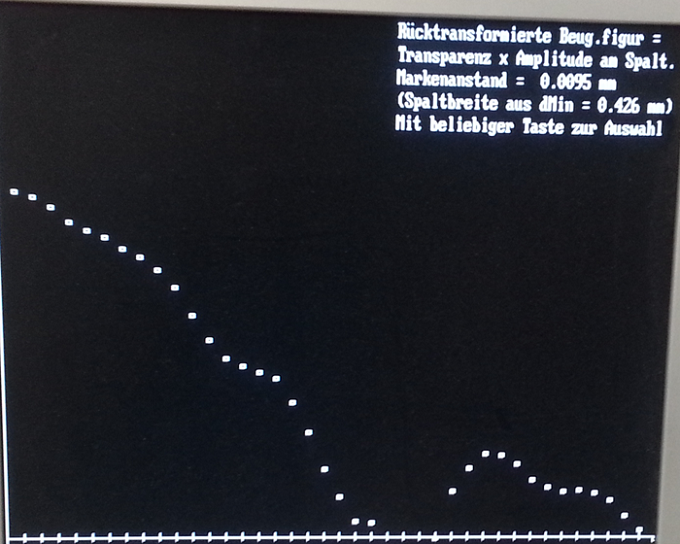
\includegraphics[width=0.8\textwidth]{bilder/aufgabe1.png}\\
	\end{tabular}
	\caption{Bild des Spaltes}
	\label{fig:aufgabe1}
\end{figure}
Mithilfe eines \emph{FFT}-Programms auf dem Computer haben wir das Spaltbild zurückgewinnen können (s. Abbildung \ref{fig:aufgabe1}). Die berechnete Spaltbreite betrug $\unit[0.426]{mm}$, das ist eine Abweichung von $\unit[6.5]{\%}$ gegenüber des vom Hersteller mit $\unit[0.4]{mm}$ angegebenen Wertes.
\section{Michelson-Interferometer}
In dieser Versuchsreihe werden wir den Interferometer für verschiedene Messungen anwenden.
\subsection{Bestimmung des Magnetostriktionskoeffizienten}
Am beweglichen Spiegel des Interferometers haben wir den von einer Spule umschlossenen Nickelstab befestigt. Legt man einen elektrischen Strom in der Spule an, so wird ein magnetisches Feld induziert, dass eine Längenänderung des Stabes bewirkt (Magnetostriktion). Ändert man den Strom ständig, so ändert sich auch die Länge des Stabes, welche wiederum das Interferenzbild auf dem Schirm ändert.\\ \\
Es war die Magnetrostriktivekonstante $\alpha$ zu bestimmen. Laut Vorbereitung könnte man sie anhand folgender Formel bestimmen:
\begin{equation}
\alpha \cdot I = \frac{m \cdot \lambda}{2 n}
\end{equation}
wobei $m$ die Anzahl der Minimum-Minimum Durchgänge, $I$ der gemessene Strom, $n=2000$ die Windungszahl der Spule und $\lambda=\unit[632.8]{nm}$ die Wellenlänge des Lasers.\\ \\
Die Konstante $\alpha$ bestimmt man also aus der Steigung der Ausgleichsgerade, die man erhält, wenn man $I$ über $\frac{m \cdot \lambda}{2n}$ aufträgt.
Wir variierten den Strom (um mehr Werte zu bekommen, haben wir beide Stromrichtungen ausprobiert) und notierten dabei die Hell-Dunkel bzw. Minima-Maxima Durchgänge. Nach Auftragen der Werte erhalten wir folgendes Schaubild:
\begin{figure}[H]
	\centering
	\begin{tabular}{@{}r@{}}
		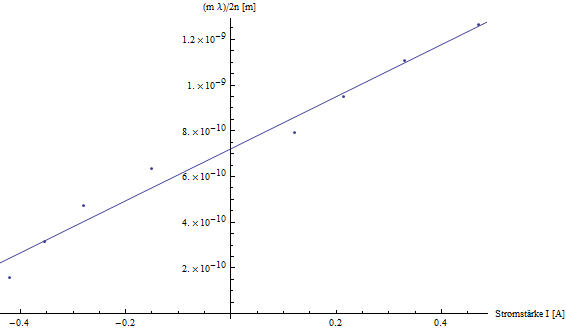
\includegraphics[width=0.6\textwidth]{bilder/aufgabe21.png}\\
	\end{tabular}
	\caption{Ausgleichsgerade zur Bestimmung der Magnetostriktionskonstante $\alpha$}
	\label{fig:aufgabe21}
\end{figure}
Aus der Steigung der Ausgleichsgerade ergibt sich die gesuchte Magnetostriktionskonstante $\alpha$:
\begin{equation*}
\alpha=\unit[1.13793 \cdot 10^{-9}]{\frac{m}{A}}
\end{equation*}
\subsection{Wellenlänge des Laserlichts}
Es soll nun die Wellenlänge des Laserlichts bestimmt werden. Wir nutzten hierfür ein anderes Interferometer als im anderen Versuch, dessen Wellenlänge wir kannten. Wir haben dann nach  jedem 10. Maximum-Maximum-Durchgang den Spiegel ein wenig verstellt und ihre Position festgehalten. Tabelle \ref{tab:aufgabe22} fasst unsere Daten zusammen:
\begin{table}[H]
\begin{tabular}{c|c}
	Maxima Durchgänge $m$ & Verschiebung $[\mu m]$ \\
	\hline
	18 & 5 \\
	28 & 7.5 \\
	38 & 10 \\
	48 & 12.2 \\
	58 & 14.9 \\
	68 & 17.2 \\
	78 & 20.1 \\
\end{tabular}
\caption{Messungen zur Bestimmung der Wellenlänge}
\label{tab:aufgabe22}
\end{table}
Diese Daten reichen laut unserer Vorbereitung aus, um die Wellenlänge zu bestimmen:
\begin{equation}
\Delta l = \lambda \frac{m}{2} \quad \Rightarrow \quad 2 \Delta l = \lambda m
\end{equation}
Wir tragen $2 \Delta l$ über $m$ auf, machen wir eine lineare Regression und aus der Steigung der Gerade erhalten wir die Wellenlänge $\lambda=\unit[497]{nm}$.
\begin{figure}[H]
	\centering
	\begin{tabular}{@{}r@{}}
		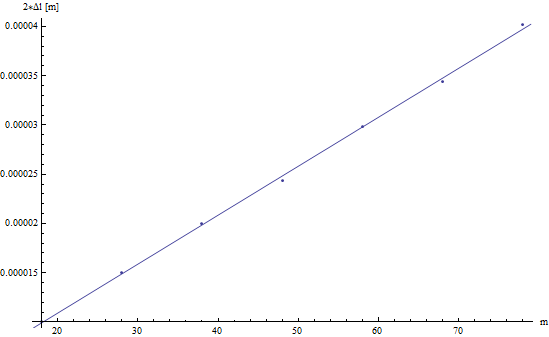
\includegraphics[width=0.8\textwidth]{bilder/aufgabe22.png}\\
	\end{tabular}
	\caption{Ausgleichsgerade zur Bestimmung der Wellenlänge $\lambda$}
	\label{fig:aufgabe22}
\end{figure}
\subsection{Demonstration des Dopplereffekts}
\subsubsection{Bei Lichtwellen mit $v \approx c$}
Hier wurde der Spiegel mit einem Motor langsam bewegt, dabei war der Motor über einen Riemen mit der Drehschraube verbunden. Es war darauf zu achten, dass genügend Spannung auf dem Riemen war und dass der Motor eine Zeit laufen muss bevor er die gewünschte Geschwindigkeit hat.\\
Wir beobachten die Durchgänge und notierten deren Anzahl alle 15 Sekunden. Im Anschluss führten wir die selbe Messung durch und notiert dabei die zurück gelegte Strecke:
 
\begin{table}[H]
\centering
\caption{Dopplereffekt}
 \begin{tabular}{c|c|c}
   $\Delta t$ in s & Anzahl der Durchgänge $n$ & zurückgelegte Strecke $\Delta s$ in $\mu m$ \\
  \hline
  15 & 15 & 5\\
  30 & 15 & 5\\
  45 & 16 & 5\\
  60 & 15 & 5.5\\
  75 & 15 & 5\\
  90 & 16 & 5.5\\
  105 & 16 & 5\\
  120 & 16 & 5\\
  135 & 17 & 5.2\\   
 \end{tabular}
\end{table}
 
Mit Mittelwert der Durchgänge $\overline{n}=15.7$ ergibt sich für die Geschwindigkeit:
 
\begin{equation*}
v= \frac{m \cdot \lambda}{2 \cdot \Delta t} = \unit[260]{\frac{nm}{s}}
\end{equation*}
 
Mit dem Mittelwert der Weglänge $\Delta s = \unit[5.19]{\mu m}$ über den klassischen Weg:
 
\begin{equation*}
v_k= \frac{\Delta s}{\Delta t}= \unit[346]{nm}
\end{equation*}
 
Das ist eine Abweichung von $\unit[33.08]{\%}$ vom Wert den wir über die Durchgänge erhalten haben.
\subsubsection{Bei Schallwellen}
Dieser Versuch konnte nicht durchgeführt werden, da keine Stimmgabeln vorhanden waren. Wobei wir aus (schulischer und Alltags-) Erfahrung wissen, dass ein Frequenzunterschied hörbar ist.
\section{Faraday-Effekt und Pockels-Effekt}
\subsection{Intensitätsmodulation anhand des Faraday-Effekts}
Dieser Versuch wurde wie in der Vorbereitung und auf dem Aufgabenblatt aufgebaut und durchgeführt: Wir stellten Bleisilikatglas in der Spule, als Modulator in den Laserstrahl. Über einen MP3-Player wurde dann die Spannung in der Spule Moduliert (und damit das Magnetfeld). Ein Photoelement das mit einem Lautsprecher gekoppelt war interpretiert das ankommende Signal (Intensität des Laserstrahls).\\
Insgesamt war ein überraschend deutliches Signal (Musik) zuhören, wenn auch mit Störgeräuschen. Wie in der Vorbereitung bereits vermutet konnten höhere Frequenzen nicht wahrgenommen werden.
\subsection{Bestimmung der Verdetschen Konstante von Bleisilikatglas}
In diesem Versuch bestimmen wir die Verdetsche Konstante $V$ und nutzen dazu die Beziehung aus der Vorbereitung:

\begin{equation*}
V = \frac{\alpha}{\mu_0 N \cdot I}
\end{equation*}

Wir haben die Polarisationswinkel $\alpha$ für verschiedene Stromstärken bestimmt, von $\unit[0]{A}$ bis $\unit[3]{A}$ bzw. $\unit[-]{A}$ (umgekehrte Stromrichtung) in $\unit[1]{A}$-Schritten. Dabei wurde der Analysator immer wieder so nachjustiert, dass es zu einem Minimum kam. Dann haben wir zur Bestimmung von $V$ den Winkel $\alpha$ über der Stromstärke $I$ aufgetragen und eine lineare Regression durchgeführt.\\ \\

\begin{figure}[H]
\centering
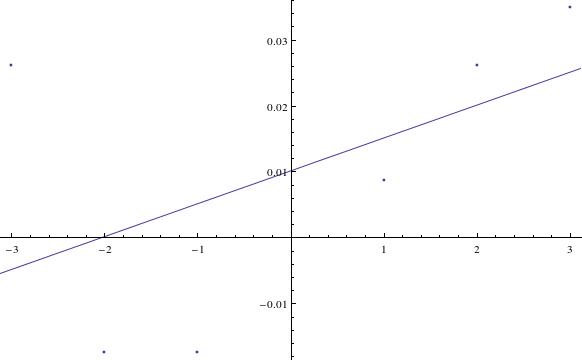
\includegraphics[scale=.3]{bilder/aufgabe32.jpg} 
\caption{Lineare Regression für Faraday-Effekt}
\end{figure}

Die Steigung $\frac{\alpha}{I}$ kann, dann in die obige Formel für $V$ eingesetzt werden und wir erhalten:

\begin{equation*}
V = \frac{\alpha}{\mu_0 N \cdot I} = \unit[0,00499]{\frac{rad}{A}} \cdot \frac{1}{4\pi \cdot \unit[10 ^{-7}]{\frac{N}{A^2}}*800}= \unit[4.9636]{\frac{rad}{Tm}}
\end{equation*}

Dabei muss der Wert für $\frac{\alpha}{I}$ in $\frac{rad}{A}$ umgerechnet werden.
\subsection{Intensitätsmodulation anhand des Pockel-Effekts}
Dieser Versuch wurde nicht durchgeführt.
\subsection{Konstantenbestimmung $k=\Delta n(E)$ für $LiNbO_3$}
In diesem Versuch gehen wir ähnlich wie bei der Bestimmung der Verdetschen Konstante. Wir variieren hier allerdings die Spannung und zwar von $\unit[-2000]{V}$ bis $\unit[2000]{V}$ in dem wir die Stromrichtung umdrehen. Wir suchten uns eine Referenzstelle und notierten die Spannungswerte bei denen es zu einem Extrem (Minimum und Maximum) kam. Die Extrema wurden, dann wie in der Vorbereitung durch nummeriert und die Nummern über die Spannung aufgetragen. Die Steigung der entstehenden Geraden ergibt die Halbwertspannung $U_{HW}$ mit welcher sich die gesuchte Konstante errechnen lässt.\\
Der Versuch wurde von allen Gruppen zusammen durchgeführt, da zu wenige Pockels-Zellen vorhanden waren.

\begin{figure}[H]
\centering
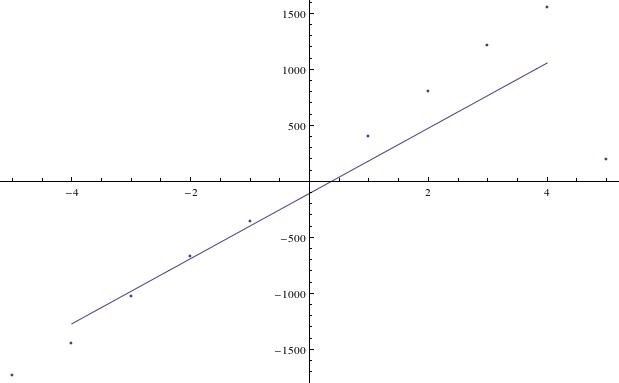
\includegraphics[scale=.7]{bilder/aufgabe34.jpg} 
\caption{Lineare Regression für Pockels-Effekt}
\end{figure}

Wir erhielten für die Halbwertsspannung $U_{HW}= \unit[290.94]{V}$. Damit ergibt sich:

\begin{equation*}
k= \frac{\lambda_0 \cdot d}{2s \cdot U_{HW}}= \frac{\unit[497]{nm} \cdot \unit[2]{mm}}{2 \cdot \unit[20]{mm} \cdot \unit[290.94]{V}} = \unit[0,0854]{\frac{nm}{V}}
\end{equation*}
\section{Optische Aktivität}
\subsection{Spezifisches optisches Drehvermögen einer Zuckerlösung}
In diesem Teil des Praktikums haben wir uns mit chiralen Stoffen beschäftigt, im Konkreten mit Haushaltszucker und Sorbose. Dabei sollte der spezifische Drehwinkel und Drehsinn der Stoffe bestimmt werden. Die Sorboselösung war bereits fertig vorhanden, die Haushaltszuckerlösung stellten wir selbst her.\\
Wie aus der Vorbereitung bereits bekannt, gilt für den spezifischen Drehwinkel:

\begin{equation*}
[\alpha] = \frac{\alpha}{c \cdot l}
\end{equation*}

Mit der Konzentration der Lösung $c$ und der Weglänge durch die Lösung $l$. Die Haushaltszuckerlösung wurde in einer quaderförmigen Küvette angerührt, wobei wir bei einer Konzentration von $c = \unit[0,3]{\frac{g}{{cm}^3}}$ begannen. Es wurde jeweils eine Messung längs und quer der Küvette durchgeführt und dann die Konzentration durch Zugabe von Wasser verändert (bzw. verringert). Für die Startkonzentration haben wir leider nur einen Wert längs der Küvette.\\
Unsere Messungen ergaben für den Haushaltszucker:

\begin{table}[H]
\centering
\begin{tabular}{c|c|c|c}
	Konzentration $c$ in $\frac{g}{{cm}^3}$ & Weglänge $l$ in $dm$ & Winkel $\Delta \alpha$ & $[\alpha]$ in $\frac{^\circ \cdot {cm}^3}{g \cdot dm}$ \\
	\hline
	0.3 & 1.98 & 10 & 16,84\\
	0.15 & 1.98 & 6 & 20,20\\
	0.15 & 0.58 & 1 & 11,49\\
	0.1 & 1.98 & 3,5 & 17,68\\
	0.1 & 0.58 & 1 & 17,24\\
	0.088 & 1.98 & 3 & 17,68\\
	0.088 & 0.58 & 1 & 20,12\\
\end{tabular}
\caption{Messungen Haushaltszucker}
\label{tab:aufgabe41}
\end{table}


Damit ergibt sich ein Mittelwert von $\overline{[\alpha]} = \unit[17.32]{\frac{^\circ \cdot {cm}^3}{g \cdot dm}}$. Allerdings weichen hier unsere Werte recht stark von einander ab. Dies könnte einer unvollständigen Durchmischung der Lösungen liegen.
\subsection{Spezifisches optisches Drehvermögen einer Sorboselösung}
Für die Sorbose-Lösung gingen wir analog vor, wobei wir allerdings die Konzentration nicht veränderten. Allerdings haben wir es auch hier verpasst eine Messung quer der Küvette durchzuführen, weshalb wir nur einen Wert für $[\alpha]$ bekommen haben:

\begin{table}[H]
\centering
\begin{tabular}{c|c|c|c}
	Konzentration $c$ in $\frac{g}{{cm}^3}$ & Weglänge $l$ in $dm$ & Winkel $\Delta \alpha$ & $[\alpha]$ in $\frac{^\circ \cdot {cm}^3}{g \cdot dm}$ \\
	\hline
	0.33 & 1.98 & -37 & - 56.63\\
\end{tabular}
\caption{Messungen Haushaltszucker}
\label{tab:aufgabe41}
\end{table}

Da es sich um Einzelwert handelt kann man schlecht sagen wie aussagekräftig dieser ist, allerdings lässt sich eindeutig feststellen, dass die Sorbose-Lösung links drehend, währen die Haushaltszucker-Lösung rechtsdrehend ist. Dies entspricht auch unserer Erwartung.

\end{document}